\begin{tikzpicture}
	\draw(0,0) node [anchor=south west,inner sep=0] (image){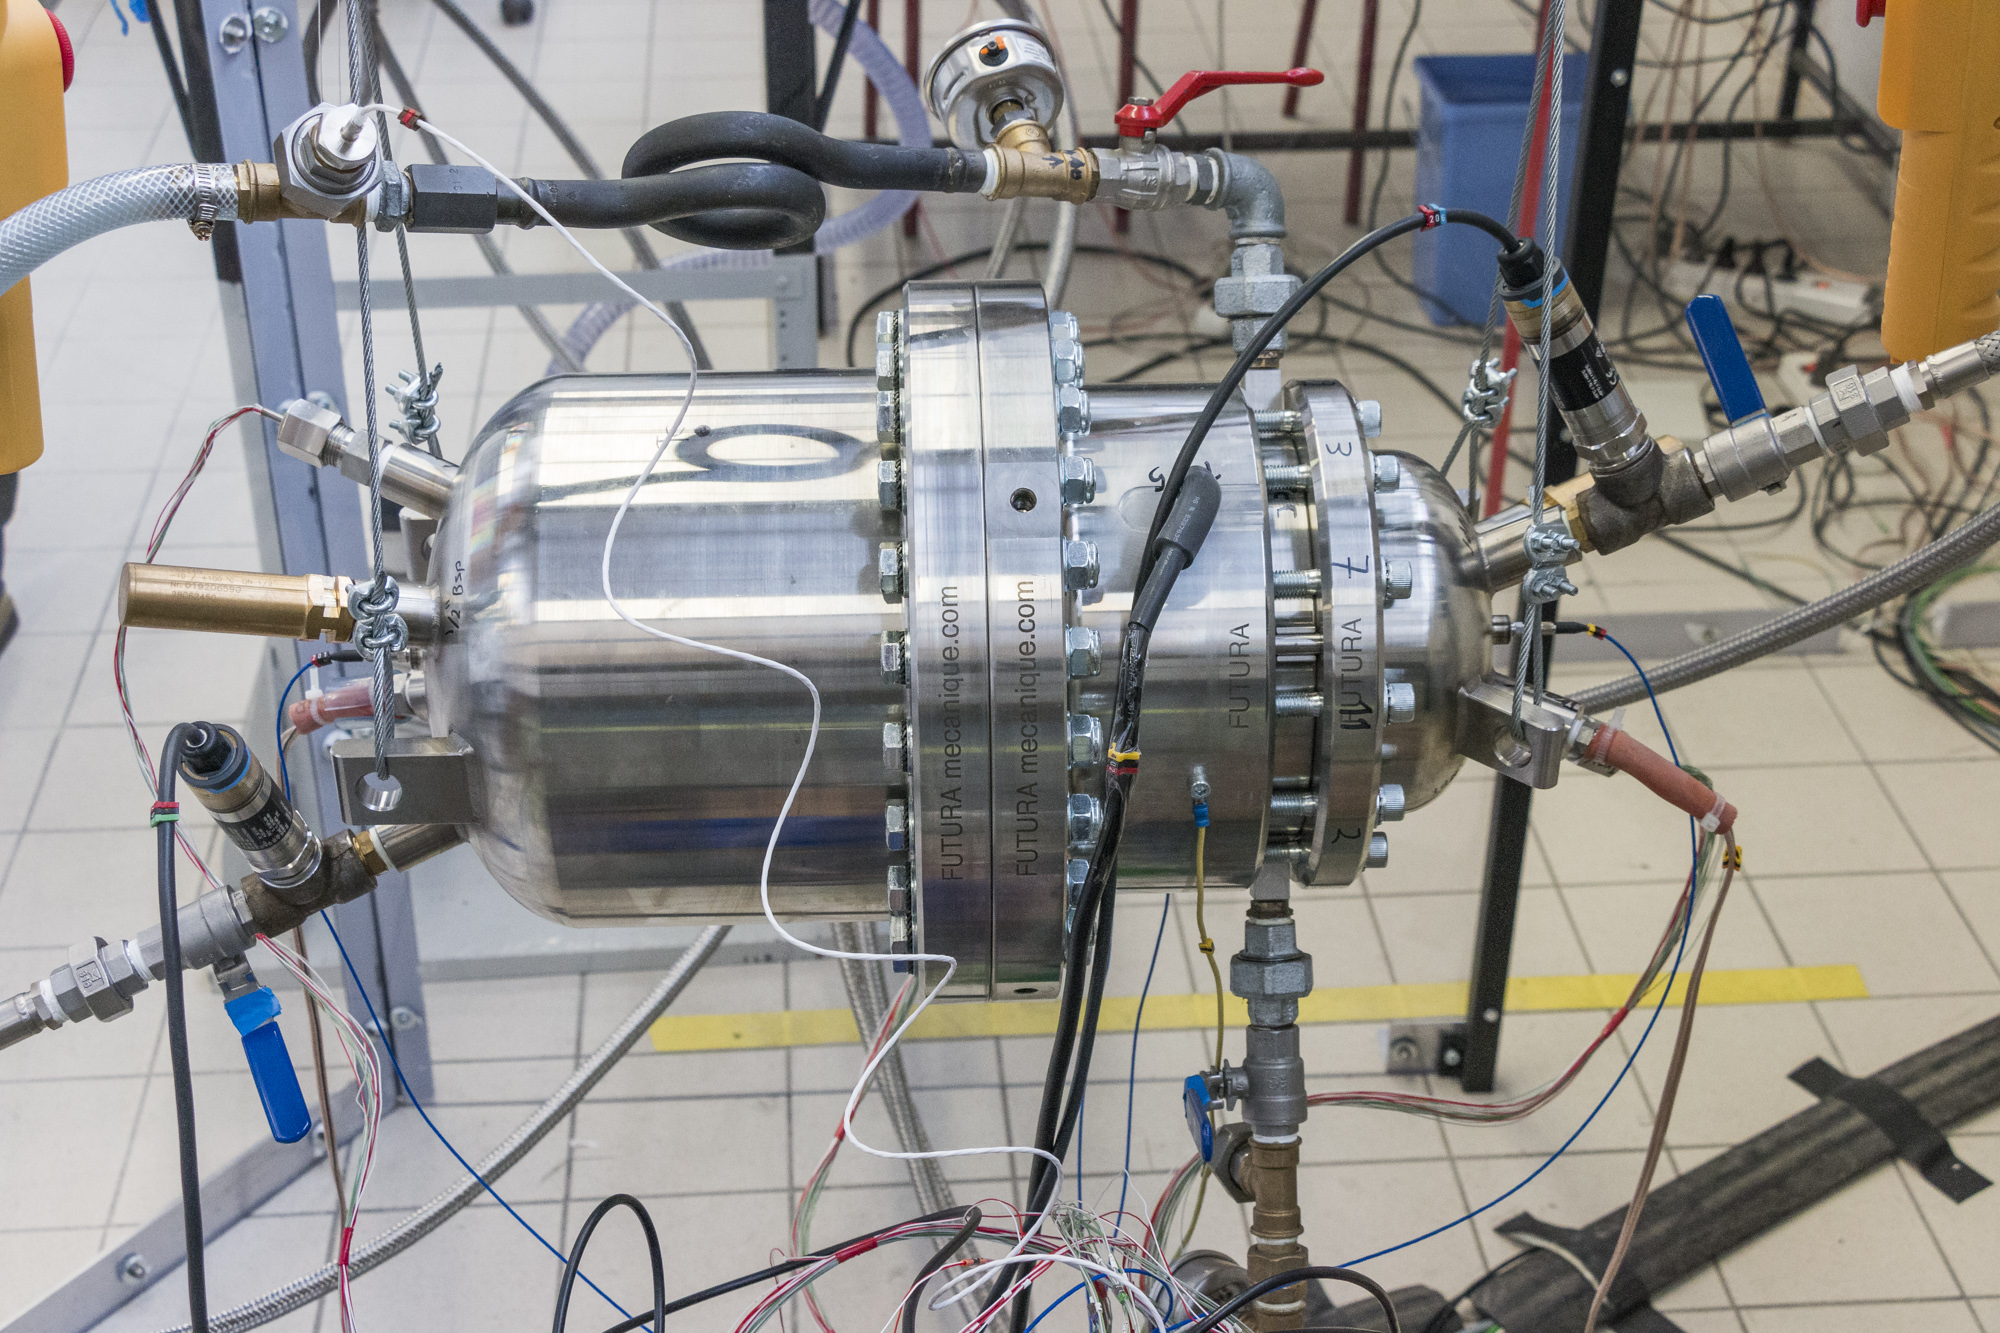
\includegraphics[width=.7\textwidth]{../fig/fig_TacotPhotos/TacotSeul_RIXGauche.jpg}};
	\begin{scope}[x={(image.south east)},y={(image.north west)}]
%		\draw[help lines, xstep=.1, ystep=.1] (0,0) grid (1,1);
		
		\draw[line width=1mm, red, rounded corners] (.07,.47) rectangle (.17,.3) node[below left, fill=white, fill opacity=.5, text opacity=1]{(b)} (.73,.85) rectangle (.85,.6) node[above right, fill=white, fill opacity=.5, text opacity=1]{(b)};
		\draw[line width=1mm, blue, rounded corners] (.13,.54) rectangle (.22,.48) node[above right, fill=white, fill opacity=.5, text opacity=1]{(a)} (.74,.55) rectangle (.83,.5) node[below left, fill=white, fill opacity=.5, text opacity=1]{(a)} (.54,.3) rectangle (.59,.35) node[above left, fill=white, fill opacity=.5, text opacity=1]{(a)};
	\end{scope}
\end{tikzpicture}